\documentclass[aspectratio=1610]{beamer}
\usepackage[T1]{fontenc}
\usetheme{wildcat}

\usepackage{amsmath,amssymb,amsfonts}
\usepackage{booktabs}
\usepackage{relsize}

\usepackage[style=verbose,backend=biber]{biblatex}
\addbibresource{main.bib}
\let\oldfootnotesize\footnotesize
\renewcommand*{\footnotesize}{\oldfootnotesize\tiny}

\def\mathdefault#1{#1}
\everymath=\expandafter{\the\everymath\displaystyle}


\title{Measurement Uncertainty, \\ Accuracy, and Precision\\
       {\small\it NE 648 - Lecture 1}}

\date{\input{term.txt} \\ {\footnotesize Git SHA: \input{git_sha.txt}}}

\author{Jeremy Roberts}



\begin{document}

\begin{frame}
\titlepage
\end{frame}

% \begin{frame}{Table of Contents}
%     \tableofcontents
% \end{frame}

\begin{frame}{}

\begin{quote}
\textcolor{wcprimary}{The principle of science, the definition, almost, is the following: {\it The test of knowledge is experiment}. Experiment is the {\it sole judge} of scientific `truth.'}
\end{quote}
\hfill  -Richard Feynman\footfullcite{feynman2015feynman} 

\vfill

\pause 

An experiment is {\it incomplete} without first analyzing the uncertainty of a reported result. \pause  Such an analysis helps to answer 
\begin{itemize}
    \item[$\ldots$] do the results agree with the theory?
    \item[$\ldots$] are the results reproducible?
    \item[$\ldots$] has a new phenomenon been observed?
\end{itemize}

\end{frame}

\begin{frame}{The Goals of Error Analysis}

\begin{enumerate}
    \item Characterize the ``spread'' observed in measurements.
    \item Identify how to improve experiments.
\end{enumerate}

\end{frame}



\begin{frame}{Example: $N_A$}

Consider the following values (in mol$^{-1}$) for Avogadro's number\footfullcite{mohr2012codata, tiesinga2021codata}:
\begin{align*}
  N_A  \begin{cases}
      \approx 6.022\cdot 10^{23} & \text{common approximation} \\
      = 6.02214129\textcolor{wcalerted}{(27)}\cdot 10^{23} & \text{2010 CODATA} \\
      = 6.02214076    \cdot 10^{23} & \text{2018 CODATA}  \\
  \end{cases} \, .
\end{align*} 
\pause  
\vfill 

Note the special notation:
 
\begin{equation*}
    6.02214129(27)\cdot 10^{23} = 
     \overbrace{6.022141\textcolor{wcalerted}{29}\cdot 10^{23}}^{\text{best estimate}} \pm \overbrace{0.000000\textcolor{wcalerted}{27}\cdot 10^{23}}^{\text{(standard) error}} \, .
\end{equation*}

\end{frame}

\begin{frame}{Uncertainties in Measurements}

If our
{\bf measurand}\footnote{the quantity intended to be measured}
is $x$,  our
{\bf best estimate}\footnote{qualitatively, a single number as ``close'' to $x$ as we can get with our measurements (usually an average)}
from one or more measurements $x_1, x_2, \ldots$ is $\bar{x}$, and $\epsilon$ is the
{\bf standard error}\footnote{qualitatively, a single number that defines ``close''},
then the statement
\begin{equation*}
x = \bar{x} \pm \epsilon
\end{equation*}
suggests that $x$ is
 
\vspace{0.25cm}

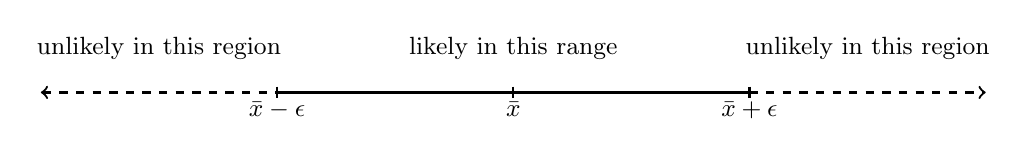
\begin{tikzpicture}[scale=1.5, every node/.style={font=\small}]
    % Mark the center point (\bar{x})
    \node[below] at (0,0) {$\bar{x}$};
    \draw[thick] (0,0.05) -- (0,-0.05);
    
    % Mark \bar{x} - \epsilon and \bar{x} + \epsilon
    \node[below] at (-2,0) {$\bar{x} - \epsilon$};
    \node[below] at (2,0) {$\bar{x} + \epsilon$};
    \draw[thick] (-2,0.05) -- (-2,-0.05);
    \draw[thick] (2,0.05) -- (2,-0.05);
    
    % Draw the interval
    \draw[thick] (-2,0) -- (2,0);
    
    % Label the range where x is likely
    \node[above] at (0,0.2) {likely in this range};
    
    % Label the unlikely regions
    \node[above] at (-3,0.2) {unlikely in this region};
    \node[above] at (3,0.2) {unlikely in this region};
    
    % Draw dashed lines outside the range
    \draw[<-, dashed, thick] (-4,0) -- (-2,0);
    \draw[->, dashed, thick] (2,0) -- (4,0);
\end{tikzpicture}

\vfill 
\pause 

We will learn how to quantify ``likely'' and ``unlikely'' with {\bf confidence intervals}.

\end{frame}


\begin{frame}{A First Experiment}

\end{frame}


\begin{frame}{Some Terminology}

First, a \textcolor{wcalerted}{warning}: ``uncertainty'' and ``error'' are often used interchangeably and ambiguously.

\pause
\vfill

However, measurements can be characterized by {\bf accuracy} and {\bf precision}:

\pause
\begin{itemize}
 \item {\it accurate} measurements yield a best estimate that ``agrees'' with an ``accepted'' value (which may not exist!)
 \pause
 \item {\it precise} measurements exhibit a ``small'' spread about the best estimate.
\end{itemize}



\end{frame}


\begin{frame}{Precision vs. Accuracy}

\begin{figure}[h!]
    \centering
    \resizebox{\textwidth}{!}{\input{figures/accuracy_vs_precision.pgf}}
\end{figure}

\vfill

\pause

Imprecision (or spread) is driven by {\bf random errors}, while inaccuracy (or {\bf bias}) is driven by {\bf systematic errors}.

\end{frame}


\begin{frame}{Whence the Spread?}

Sources of {\bf random} or {\bf aleotoric  errors} are
\begin{enumerate}
 \item technical (experimental apparatus/procedure)
 \item fundamental noise (laws of physics)
\end{enumerate}


\vfill
\pause

Technical noise can, in theory, be reduced by modifying an experimental apparatus or procedure, but left unchanged, {\it random errors are generally irreducible}!

\vfill
\pause

The spread (of repeated measurements) about a best estimate is usually quantified statistically with the {\bf (sample) standard deviation}.

\vfill
\pause

If ({\it and only if}) repeated measurements with a device are identical, the measurement precision is the device precision, i.e.,
\begin{itemize}
 \item a half division if the device is {\bf analog} (e.g., ruler, dial)
 \item one in the last digit if the device is {\bf digital} (e.g., display on balance)
\end{itemize}

\end{frame}


\begin{frame}{Possible Sources of Random Errors}

\begin{enumerate}
 \item electronic noise when measuring a signal with an oscilloscope
 \item varied use of a survey meter by different individuals
 \item finite resolution of a digital display on a mass balance
 \item cosmic radiation during a count
 \item apparent fluctuations in low-light or low-current signals
 \item apparent fluctuations of pair-formation energy in a radiation detector
\end{enumerate}

\vfill

Which of these are technical?  fundamental?

\end{frame}


\begin{frame}{Whence the Inaccuracy?}

Sources of {\bf systematic} or {\bf epistemic  errors} include
\begin{enumerate}
 \item miscalibrated equipment
 \item misused equipment
 \item incorrect physics models
 \item (other) mistakes
\end{enumerate}

\vfill
\pause

Systematic error are hard to identify and quantify---why?


\end{frame}


\begin{frame}{Common Systematic Errors}


\begin{enumerate}
 \item zero errors (e.g., forgetting to rezero a scale; ruler with offset zero...)
 \item calibration errors (e.g., using a wrong check source to calibrate the HPGe)
 \item insertion errors (e.g., inserting room-temperature thermometer into small volume of hot liquid)
\end{enumerate}

\vfill

Can you think of others?

\vfill

\end{frame}


\begin{frame}{Summary}

\begin{itemize}
 \item An experiment is incomplete without an error analysis.
 \item Measurements exhibit random errors and systematic errors.
 \item A high precision means a small random error (or spread).
 \item A high accuracy means a small systematic error.
 \item Random errors can be characterized by statistics (of repeated measurements).
 \item Systematic errors are hard to identify and characterize.
\end{itemize}


\end{frame}


\end{document}

